This chapter will provide in its first part a detailed analysis of the system functionalities, in order to estimate the size of the project in terms of LOC, using the FP approach. Instead, in the second part, we will use the COCOMO approach to estimate costs and efforts.
\section{Size estimation using FP}
For the FP estimation, we will use the IFPUG standard, so we will divide the analysis into 5 categories (ILF, ELF, EI, EQ, EO), and for each of them, provide a list of functions to be developed and their expected complexity. We will also present all the tables we used to estimate these values.

\subsection{Internal Logic Files (ILF)}
The ILF definition by IFPUG is: \bigbreak
\textit{"An ILF is a user-identifiable group of logically related data or control information maintained within the boundary of the application. The primary intent of an ILF is to hold data maintained through one or more elementary processes of the application being counted."} \bigbreak
So, we will consider ILF all our data structures that resides inside the system itself. The tables used to estimate complexity and FP are quoted below.

\begin{figure}
  \centering
  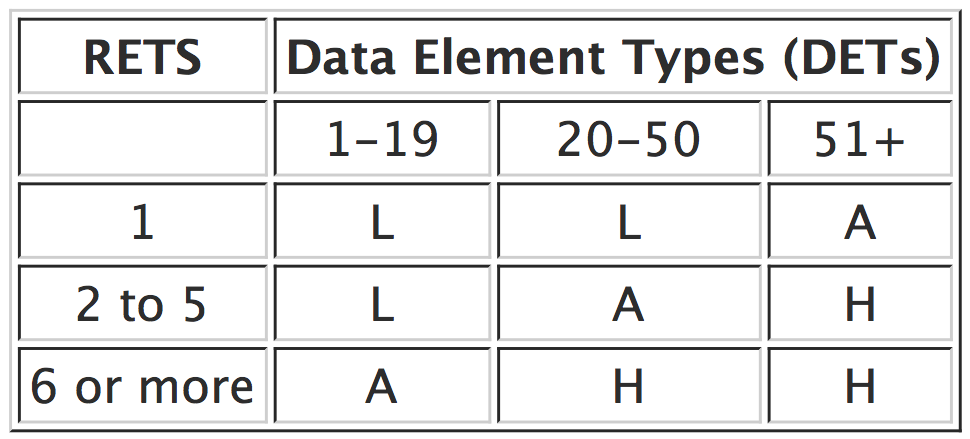
\includegraphics[width=0.5\textwidth]{ILFcomp}
  \caption{Complexity estimation for ILF}
\end{figure}

All the ILF that we have identified are:
\begin{itemize}
\item \textbf{Drivers (extension of users):} we identified 6 DET (email, pwd, birthdate, status, license-info, payment-info) and 3 RET (valid drivers, no license drivers, no payment drivers). So we will consider it \textbf{LOW}.
\item \textbf{Workers (extension of users):} we identified 6 DET (name, pwd, rfid, status, position, notification) and 2 RET (active workers, inactive). We will consider it \textbf{LOW}.
\item \textbf{Admins (extension of users):} we identified 3 DET(username, pwd, 2faseed). We will consider it \textbf{LOW}.
\item \textbf{Vehicle:} we identified 6 DET (plate, status, battery, position, last-interaction, current-drive-id, issue) and 3 RET (in use, maintenance, available). We will consider it \textbf{LOW}.
\item \textbf{Reservation:} we identified 3 DET(vehicle, timestamp, driver). We will consider it \textbf{LOW}.
\item \textbf{Drive:} we identified 13 DET(vehicle, driver, reservation, start-timestamp, stop-timestamp, start-position, stop-position, length, occupants, last-battery, report, amount, discounts) and 5 RET (driving, stopped, payed, with report, with discounts). We will consider it \textbf{AVG}.
\item \textbf{Payment:} we identified 5 DET (user, drive, timestamp, amount, method). We will consider it \textbf{LOW}.
\item \textbf{Task:} we identified 5 DET (worker, vehicle, timestamp, description, priority). We will consider it \textbf{LOW}.
\end{itemize}

\begin{figure}
  \centering
  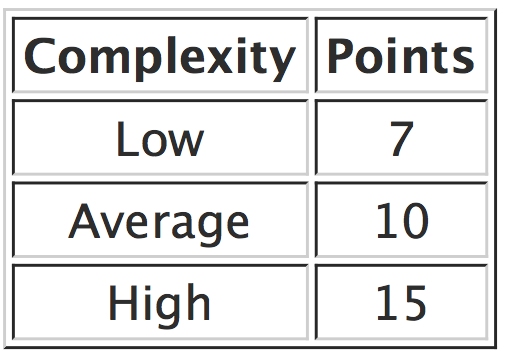
\includegraphics[width=0.25\textwidth]{ILFfp}
  \caption{Function Point estimation for ILF}
\end{figure}

The total FP from ILF is then 59, as shown in the review Table 2.1. 

\clearpage

\begin{table}
  \centering
    \begin{tabular}{| l | l | l |}
    \hline
    \textbf{ILF} & \textbf{Complexity} & \textbf{FPs} \\ \hline
    Drivers & LOW & 7 \\ \hline
    Workers & LOW & 7\\ \hline
    Admins & LOW & 7\\ \hline
    Vehicle & LOW & 7\\ \hline
    Reservation & LOW & 7\\ \hline
    Drive & AVG & 10\\ \hline
    Payment & LOW & 7\\ \hline
    Task & LOW & 7\\ \hline 
    \hline
    \multicolumn{2}{|l|}{Total} & 59 \\ \hline
    \end{tabular}
  \caption{Total FP from ILF}
\end{table}



\subsection{External Logic Files (ELF)}
The ELF definition by IFPUG is: \bigbreak
\textit{"An external interface file (EIF) is a user identifiable group of logically related data or control information referenced by the application, but maintained within the boundary of another application. The primary intent of an EIF is to hold data referenced through one or more elementary processes within the boundary of the application counted. This means an EIF counted for an application must be in an ILF in another application."}
\bigbreak
The only external data we have is the vehicle state, but since it is replicated by polling inside our database, it is considered again ILF (see above). 

\subsection{External Inputs (EI)}
The EI definition by IFPUG is: \bigbreak
\textit{"An external input (EI) is an elementary process that processes data or control information that comes from outside the application boundary. The primary intent of an EI is to maintain one or more ILFs and/or to alter the behavior of the system."}
\bigbreak
We have many external input, so we will divide them per user type (as we have always done). As before, the tables used to estimate FP are copied here.
\begin{figure}
  \centering
  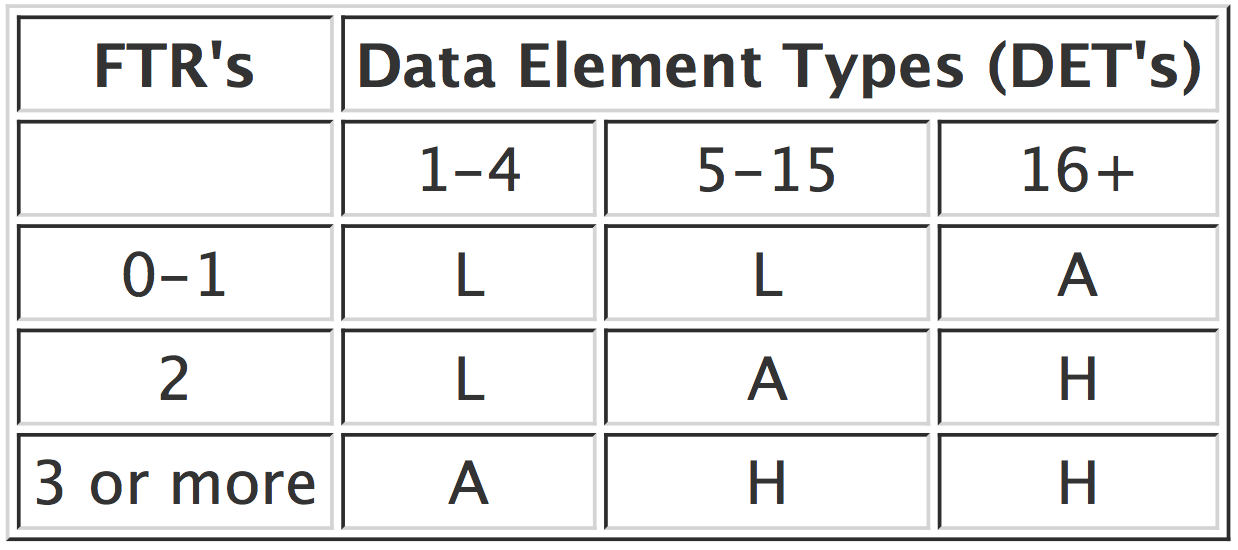
\includegraphics[width=0.5\textwidth]{EIcomp}
  \caption{Complexity estimation for EI}
\end{figure}

\subsubsection{Drivers EI}
\begin{itemize}
\item \textbf{Login/Logout:} the login phase need to access few components, and the operations of password checking (and possibly token generation) are quite standard. \textbf{LOW} complexity.
	\item \textbf{Signup:} The signup phase requires not only the insertion of the new user, but also the processing of license and payment infos. \textbf{AVG} complexity.
	
	\item \textbf{Reserve:} The reserve process access different components, need to check if a vehicle is available, check if the user has the minimum amount and check if user is authorized. \textbf{AVG} complexity.
	
	\item \textbf{Unlock:} This operation is quite simple, since it only need to send a request to the vehicle. \textbf{LOW} complexity.

	\item \textbf{CancelReservation:} This operation only requires to check that the reservation exists and if the time limit has not passed. \textbf{LOW} complexity.
	
	\item \textbf{Report:} This operations generates a report, that must be validated and then transformed into a Task possibily. \textbf{AVG} complexity. 
\end{itemize}
\subsubsection{Workers EI}
\begin{itemize}
	\item \textbf{Login:} Since the login is slightly different it will be counted again for the workers. The Logout instead is the same. \textbf{LOW} complexity.

	\item \textbf{ChangeMyState:} Only changes the state (available/ unavailable) of the worker. \textbf{LOW} complexity.
	
	\item \textbf{UpdateTask:} This operations changes the state of the task.\textbf{LOW} complexity. 
\end{itemize}
\subsubsection{Admin EI}
\begin{itemize}
	\item \textbf{Login:} Since the login is slightly different it will be counted again for the admins. The Logout instead is the same. \textbf{LOW} complexity.

	\item \textbf{ManageWorker:} Only applies to the workers dataset. \textbf{LOW} complexity.
	
	\item \textbf{MakeTask:} This operations only generates a task.\textbf{LOW} complexity. 
\end{itemize}

\begin{figure}
  \centering
  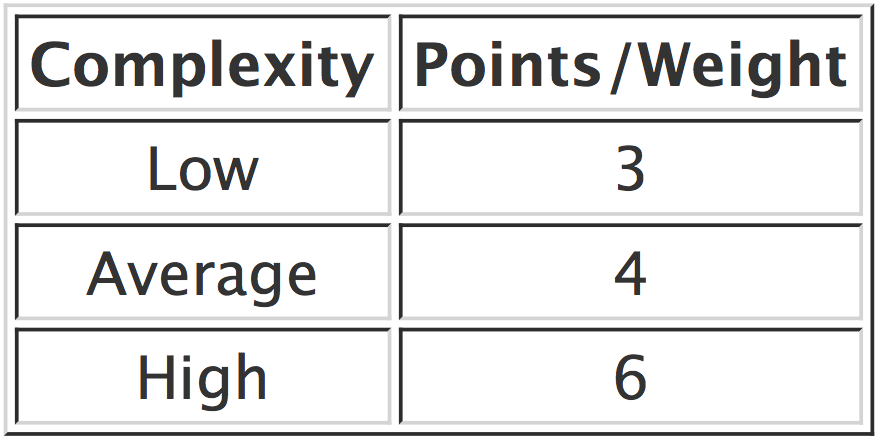
\includegraphics[width=0.35\textwidth]{EIfp}
  \caption{Function Point estimation for EI}
\end{figure}

The total FPs from EI are 41, as in the review Table 2.2.

\begin{table}
  \centering
    \begin{tabular}{| l | l | l |}
    \hline
    \textbf{EI} & \textbf{Complexity} & \textbf{FPs} \\ \hline
    Driver-Login & LOW & 3 \\ \hline
    Logout & LOW & 3\\ \hline
    Driver-Signup & AVG & 4\\ \hline
    Driver-Reserve & AVG & 4\\ \hline
    Driver-Unlock & LOW & 3\\ \hline
    Driver-CancelReservation & LOW & 3\\ \hline
    Driver-Report & LOW & 3\\ \hline
    Worker-Login & LOW & 3\\ \hline
    Worker-ChangeMyState & LOW & 3\\ \hline
    Worker-UpdateTask & LOW & 3\\ \hline
    Admin-Login & LOW & 3\\ \hline
    Admin-ManageWorker & LOW & 3\\ \hline
    Admin-MakeTask & LOW & 3\\ \hline
    \hline
    \multicolumn{2}{|l|}{Total} & 41 \\ \hline
    \end{tabular}
  \caption{Total FP from EI}
\end{table}

\clearpage

\subsection{External Outputs (EO)}
The definition of EO by IFPUG is: \bigbreak
\textit{"An external output (EO) is an elementary process that sends data or control information outside the application boundary. The primary intent of an external output is to present information to a user through processing logic other than, or in addition to, the retrieval of data or control information . The processing logic must contain at least one mathematical formula or calculation, create derived data maintain one or more ILFs or alter the behavior of the system."}
\bigbreak
\begin{figure}
  \centering
  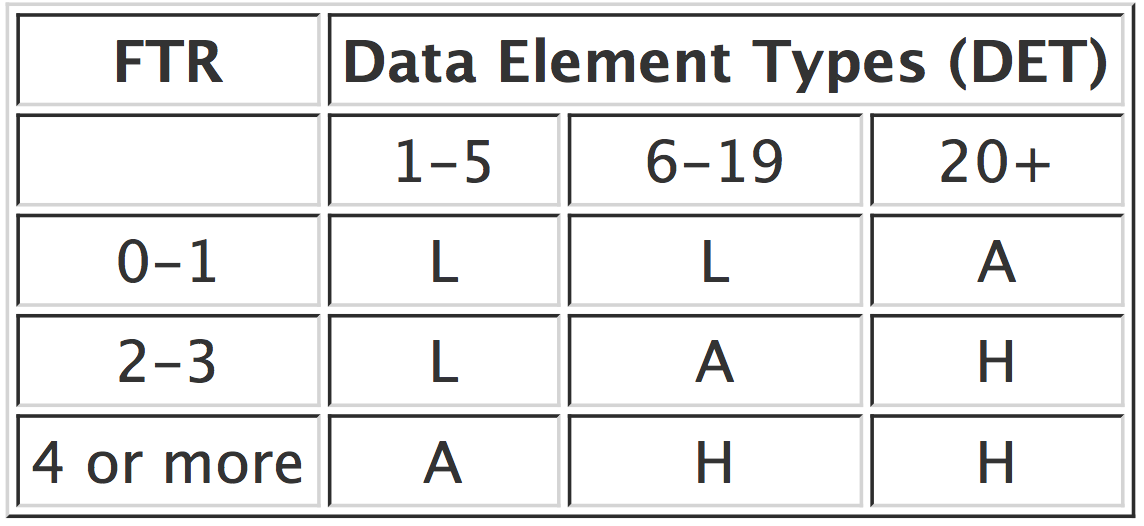
\includegraphics[width=0.5\textwidth]{EOcomp}
  \caption{Complexity estimation for EO}
\end{figure}
We only have 2 External Output, that are:
\begin{itemize}
\item \textbf{Push-Notification to Workers} Since it is only a communication of a new task assignment, we will assign \textbf{LOW} complexity to this.
\item \textbf{Vehicle Polling} Vehicle polling is another primary operation of our system, but it is quite simple. \textbf{LOW} complexity.
\end{itemize}

The resulting FPs for EO are 8, as stated in the Table 2.3.

\begin{figure}
  \centering
  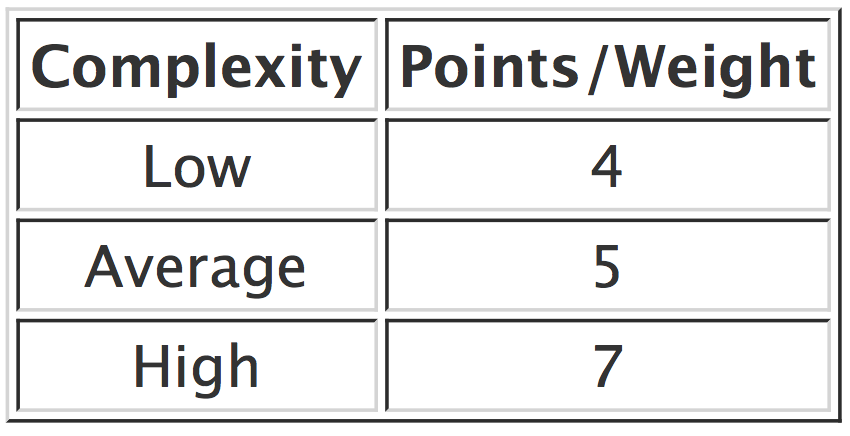
\includegraphics[width=0.35\textwidth]{EOfp}
  \caption{Function Point estimation for EO}
\end{figure}

\clearpage

\begin{table}
  \centering
    \begin{tabular}{| l | l | l |}
    \hline
    \textbf{EO} & \textbf{Complexity} & \textbf{FPs} \\ \hline
    Worker push & LOW & 4 \\ \hline
    Vehicle polling & LOW & 4\\ \hline
    \hline
    \multicolumn{2}{|l|}{Total} & 8 \\ \hline
    \end{tabular}
  \caption{Total FP from EO}
\end{table}

\subsection{External Inquiry (EQ)}
The definition of EQ by IFPUG is: \bigbreak
\textit{"An external inquiry (EQ) is an elementary process that sends data or control information outside the application boundary. The primary intent of an external inquiry is to present information to a user through the retrieval of data or control information from an ILF of EIF. The processing logic contains no mathematical formulas or calculations, and creates no derived data. No ILF is maintained during the processing, nor is the behavior of the system altered."}
\bigbreak
\begin{figure}
  \centering
  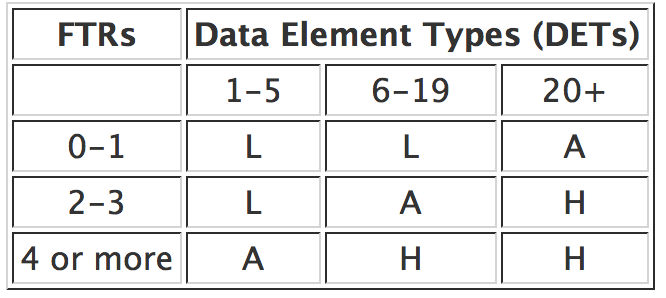
\includegraphics[width=0.5\textwidth]{EQcomp}
  \caption{Complexity estimation for EQ}
\end{figure}
We only have 2 External Inquiries, that are:
\begin{itemize}
\item \textbf{Available Vehicles:} It needs to retrieve all the available vehicles nearby a position, so it also requires a distance computation to order the vehicles. \textbf{AVG} complexity.
\item \textbf{Admin-GetStatistics:} It simply replies with the selected records given some filters, so \textbf{LOW} complexity. 
\end{itemize}

The resulting FPs for EQ are 6, as stated in the Table 2.4.

\begin{figure}
  \centering
  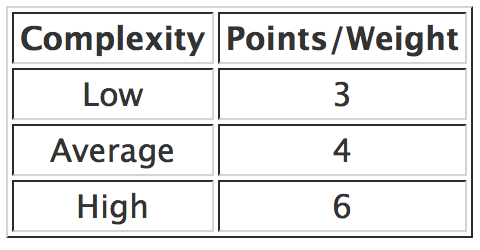
\includegraphics[width=0.35\textwidth]{EQfp}
  \caption{Function Point estimation for EQ}
\end{figure}

\begin{table}
  \centering
    \begin{tabular}{| l | l | l |}
    \hline
    \textbf{EQ} & \textbf{Complexity} & \textbf{FPs} \\ \hline
    Worker push & LOW & 3 \\ \hline
    Vehicle polling & LOW & 3\\ \hline
    \hline
    \multicolumn{2}{|l|}{Total} & 6 \\ \hline
    \end{tabular}
  \caption{Total FP from EQ}
\end{table}

\clearpage

\subsection{FP estimation recap}
The totals of every level from before is copied here and a final total is provided. 

\begin{center}
    \begin{tabular}{| l | l |}
    \hline
    \textbf{Type} & \textbf{FPs} \\ \hline
    ILF & 59 \\ \hline
    ELF & 0\\ \hline
    EI & 41\\ \hline
    EO & 8\\ \hline
    EQ & 6\\ \hline
    \hline
    \textbf{Total} & 114 \\ \hline
    \end{tabular}
\end{center}

The total of 114FPs will then be converted to SLOC using the parameter we found on the referenced website, since we are using NodeJS (and so JavaScript). The average SLOC for a FP in JS is 47. So the total SLOC of the system:
\bigbreak
\begin{center} \textbf{ SLOC = 114 * 47 = 5358} \end{center}
\bigbreak
Using instead the maximum FP to SLOC conversion rate (JS: 63) we get an upper bound of
\bigbreak
\begin{center} \textbf{ SLOC = 114 * 63 = 7182} \end{center}
\bigbreak

\clearpage
\section{COCOMO estimation}
We are going to list all our estimation on factors, and later use an online calculator compute the results. Extensive explanation of the factor types and their values are provided in the course lectures.
\subsection{Scale Drivers}
\subsubsection{Precedentedness (PREC)}
Since we have already developed different system that uses a similar architecture (NodeJS, Postgres, etc.) and there is no need for any innovative algorithm here, this factor will be set to \textbf{Very High}
\subsubsection{Development Flexibility (FLEX)}
The requirements where not so detailed and formal and where open to interpretation. Also, we had only another constraint, i.e. the API of the vehicles, that are considered already developed. We will set this to \textbf{Nominal}
\subsubsection{Architecture / Risk Resolution (RESL)} 
As stated below in our risk analysis, the dangerous risks are only few, so we are setting this to \textbf{High}
\subsubsection{Team Cohesion (TEAM)}
Since we are long-time friends and also collaborated effectively in another project, this value will be set to \textbf{Very High}
\subsubsection{Process Maturity (PMAT)}
We will opt for a Level 3 maturity (Organization Level), so \textbf{High}

\subsection{Cost Drivers}
\subsubsection{Required Software Reliability (RELY)}
Because of the design of our vehicles, we exclude any threat to human life (our system cannot stop or control a vehicle). So we are setting this to "moderate, easily recoverable losses", \textbf{Nominal}
\subsubsection{Data Base Size (DATA)}
Since our test dataset will be very small, because there are not many different situations to test, we will set this to \textbf{Low}
\subsubsection{Product Complexity (CPLX)}
We will set this to \textbf{Nominal}, because our code will user simple callbacks, middle-wares etc., and also, in mobile development, we will user device-dependant operations that are not straight-forward. 
\subsubsection{Developed for Reusability (RUSE)}
Since the components of the system are very specific to the problem, we will not take into account the Reusability of the code. The only component that could be reused is the AuthorizationManager, but it is probably better to use a third-party middleware like PassportJS instead of developing one inernally. Set to \textbf{Low}
\subsubsection{Documentation Match to Life-Cycle Needs (DOCU)}
The need of documentation is clearly fundamental, but since we are a team of 2 we will not provide a super-detailed documentation, but the right size. Set to \textbf{Nominal}
\subsubsection{Execution Time Constraint (TIME)}
Our system should interact with a lot of users together but with a not so difficult complexity. We expect a medium-high CPU usage. Set to \textbf{High}
\subsubsection{Main Storage Constraint (STOR)}
Our system won't probably need a lot of storage space, so we are leaving this to \textbf{Nominal}
\subsubsection{Platform Volatility (PVOL)}
The platform we use is composed of NodeJS (v6), Postgres (v9) that have a similar period between release (6 months for major). The vehicle on-board system instead will be updated very seldomly. Set to \textbf{Nominal}
\subsubsection{Analyst Capability (ACAP)}
Since we are not experienced analysts (requirements, design etc.) we will set this to \textbf{Low}
\subsubsection{Programmer Capability (PCAP)}
Instead we are quite good programmers, with a lot of developed team projects and a lot of lines of code. Set to \textbf{High}
\subsubsection{Personnel Continuity (PCON)}
Our team will probably remain the same, so set to \textbf{Very High}
\subsubsection{Applications Experience (APEX)}
Since we are dealing with NodeJS and SQL and we are both experienced in Android and iOS development, we will set this to \textbf{High}
\subsubsection{Platform Experience (PLEX)}
Again the team has already experience with the platform, set to \textbf{High}
\subsubsection{Language and Tool Experience (LTEX)}
Given that the tools and languages used were chosen by us, we chose the ones we have experience on. Set to \textbf{High}
\subsubsection{Use of Software Tools (TOOL)}
Since we have not a great experience with tools, but we will perform (for the first time) integration and a more formal development. Set to \textbf{Low}
\subsubsection{Multisite Development (SITE)}
Since we live in the same city, Milan, we are setting this to \textbf{Very High}
\subsubsection{Required Development Schedule (SCED)}
Given that we are not given any strong constraint on the development, we are setting this to \textbf{Nominal}
\clearpage
\subsection{Drivers recap}
Here a recap, in table form, of the choosen parameters is given: 

\begin{center}
\begin{tabular}{| l | l |}
    \hline
    \textbf{Driver} & \textbf{Value} \\ \hline
    PREC & Very High \\
    FLEX & Nominal\\ 
    RESL & High\\ 
    TEAM & Very High\\ 
    PMAT & High\\ \hline
    RELY & Nominal\\ 
    DATA & Low\\
    CPLX & Nominal\\
    RUSE & Low\\
    DOCU & Nominal\\ \hline
    TIME & High\\     
    STOR & Nominal\\
    PVOL & Nominal\\ \hline
    ACAP & Low\\
    PCAP & High\\
    PCON & Very High\\    
    APEX & High\\  
    PLEX & High\\ 
    LTEX & High\\ \hline
    TOOL & Low\\
    SITE & Very High\\   
    SCED & Nominal\\ 
    \hline
    \end{tabular}
\end{center}

\subsection{Results}
To compute the COCOMO estimation we used an online tool (referenced in Paragraph 1.3). A view of the setup is presented here, with the 2 different results provided (using both the average SLOC and maximum SLOC)

\begin{figure}
  \centering
  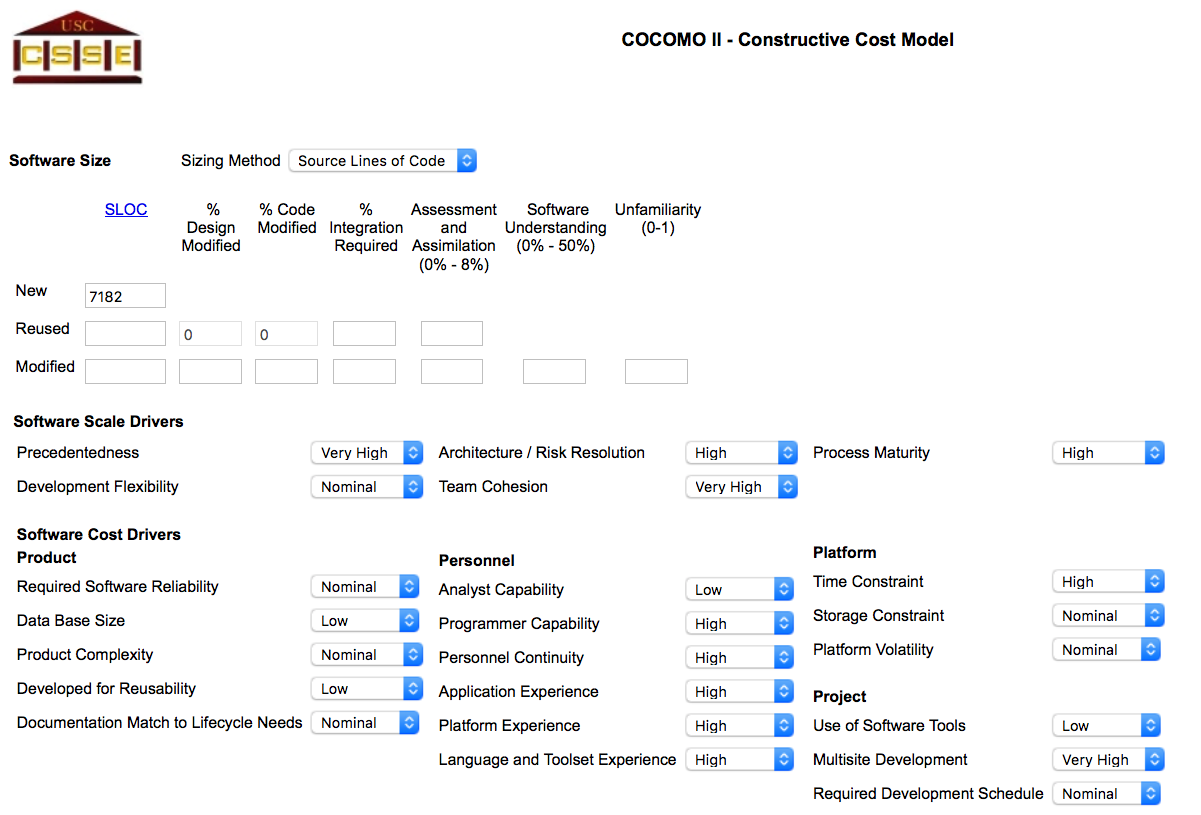
\includegraphics[width=1\textwidth]{cocohome}
  \caption{Screenshot of the online tool.}
\end{figure}

\begin{figure}
  \centering
  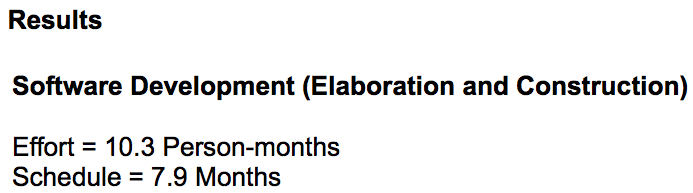
\includegraphics[width=0.6\textwidth]{cocores1}
  \caption{Results for the average SLOC.}
\end{figure}

\begin{figure}
  \centering
  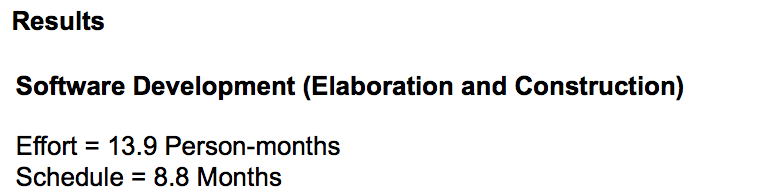
\includegraphics[width=0.6\textwidth]{cocores2}
  \caption{Results for the maximum SLOC.}
\end{figure}
